
\begin{figure}[t]
\centering
\definecolor{openarm}{HTML}{2A78D6}
\definecolor{bndarm}{HTML}{C4551F}
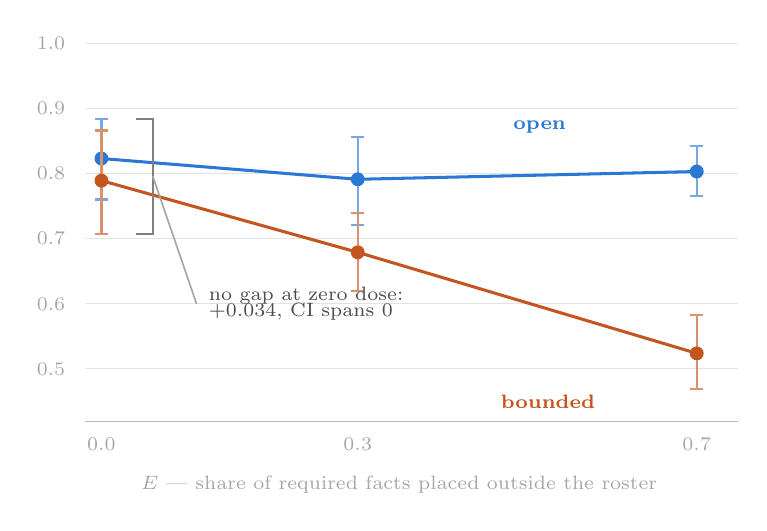
\begin{tikzpicture}[x=1.05cm,y=1.2cm,font=\small]
\draw[gray!22] (-0.2,0.552) -- (7.7,0.552);
\node[anchor=east,gray!70,font=\scriptsize] at (-0.32,0.552) {0.5};
\draw[gray!22] (-0.2,1.241) -- (7.7,1.241);
\node[anchor=east,gray!70,font=\scriptsize] at (-0.32,1.241) {0.6};
\draw[gray!22] (-0.2,1.931) -- (7.7,1.931);
\node[anchor=east,gray!70,font=\scriptsize] at (-0.32,1.931) {0.7};
\draw[gray!22] (-0.2,2.621) -- (7.7,2.621);
\node[anchor=east,gray!70,font=\scriptsize] at (-0.32,2.621) {0.8};
\draw[gray!22] (-0.2,3.310) -- (7.7,3.310);
\node[anchor=east,gray!70,font=\scriptsize] at (-0.32,3.310) {0.9};
\draw[gray!22] (-0.2,4.000) -- (7.7,4.000);
\node[anchor=east,gray!70,font=\scriptsize] at (-0.32,4.000) {1.0};
\draw[gray!55] (-0.2,0.000) -- (7.7,0.000);
\node[anchor=north,gray!70,font=\scriptsize] at (0.00,-0.080) {$0.0$};
\node[anchor=north,gray!70,font=\scriptsize] at (3.10,-0.080) {$0.3$};
\node[anchor=north,gray!70,font=\scriptsize] at (7.20,-0.080) {$0.7$};
\draw[openarm,line width=1.1pt] (0.00,2.779) -- (3.10,2.559) -- (7.20,2.641);
\draw[openarm!65,line width=.8pt] (0.00,2.345) -- (0.00,3.200);
\draw[openarm!65,line width=.8pt] (-0.08,2.345) -- (0.08,2.345);
\draw[openarm!65,line width=.8pt] (-0.08,3.200) -- (0.08,3.200);
\filldraw[openarm] (0.00,2.779) circle (2.3pt);
\draw[openarm!65,line width=.8pt] (3.10,2.076) -- (3.10,3.007);
\draw[openarm!65,line width=.8pt] (3.02,2.076) -- (3.18,2.076);
\draw[openarm!65,line width=.8pt] (3.02,3.007) -- (3.18,3.007);
\filldraw[openarm] (3.10,2.559) circle (2.3pt);
\draw[openarm!65,line width=.8pt] (7.20,2.386) -- (7.20,2.910);
\draw[openarm!65,line width=.8pt] (7.12,2.386) -- (7.28,2.386);
\draw[openarm!65,line width=.8pt] (7.12,2.910) -- (7.28,2.910);
\filldraw[openarm] (7.20,2.641) circle (2.3pt);
\draw[bndarm,line width=1.1pt] (0.00,2.545) -- (3.10,1.786) -- (7.20,0.717);
\draw[bndarm!65,line width=.8pt] (0.00,1.979) -- (0.00,3.076);
\draw[bndarm!65,line width=.8pt] (-0.08,1.979) -- (0.08,1.979);
\draw[bndarm!65,line width=.8pt] (-0.08,3.076) -- (0.08,3.076);
\filldraw[bndarm] (0.00,2.545) circle (2.3pt);
\draw[bndarm!65,line width=.8pt] (3.10,1.379) -- (3.10,2.200);
\draw[bndarm!65,line width=.8pt] (3.02,1.379) -- (3.18,1.379);
\draw[bndarm!65,line width=.8pt] (3.02,2.200) -- (3.18,2.200);
\filldraw[bndarm] (3.10,1.786) circle (2.3pt);
\draw[bndarm!65,line width=.8pt] (7.20,0.338) -- (7.20,1.124);
\draw[bndarm!65,line width=.8pt] (7.12,0.338) -- (7.28,0.338);
\draw[bndarm!65,line width=.8pt] (7.12,1.124) -- (7.28,1.124);
\filldraw[bndarm] (7.20,0.717) circle (2.3pt);
\node[openarm,anchor=south,font=\scriptsize\bfseries] at (5.3,2.941) {open};
\node[bndarm,anchor=north,font=\scriptsize\bfseries] at (5.4,0.377) {bounded};
\draw[black!50,line width=.7pt] (0.42,3.200) -- (0.62,3.200) -- (0.62,1.979) -- (0.42,1.979);
\draw[black!35,line width=.6pt] (0.62,2.593) -- (1.15,1.241);
\node[black!70,font=\scriptsize,align=left,anchor=west] at (1.18,1.241) {no gap at zero dose:\\[-2pt]$+0.034$, CI spans $0$};
\node[anchor=north,gray!70,font=\scriptsize] at (3.6,-0.480) {$E$ --- share of required facts placed outside the roster};
\end{tikzpicture}
\caption{The formation effect is reach, and the dose-response says so. \metric{E} is the
share of a task's required facts placed outside the roster; bars are 95\% percentile
bootstrap intervals over episodes. Four things hold at once, and the axis needs all four:
the contrast \textbf{vanishes at zero dose}, which is the control it had to pass; the arm
that cannot be affected is \textbf{flat} across all three doses; the mechanism variable
tracks the dose (the bounded arm's useful sources fall $4.36 \to 3.17 \to 1.26$); and
fabrication appears only as sources dry up ($0 \to 0.139 \to 0.333$ per task).}
\label{fig:dose}
\end{figure}
